  \section{Déployer OpenStack}

  \begin{frame}
    \frametitle{Ce qu'on va voir}
    \begin{itemize}
      \item Installer OpenStack à la main \url{http://docs.openstack.org/icehouse/install-guide/install/apt/content/}
      \item Donc comprendre son fonctionnement
      \item Tour d'horizon des solutions de déploiement
    \end{itemize}
  \end{frame}

  \begin{frame}
    \frametitle{Architecture détaillée}
    \begin{center}
      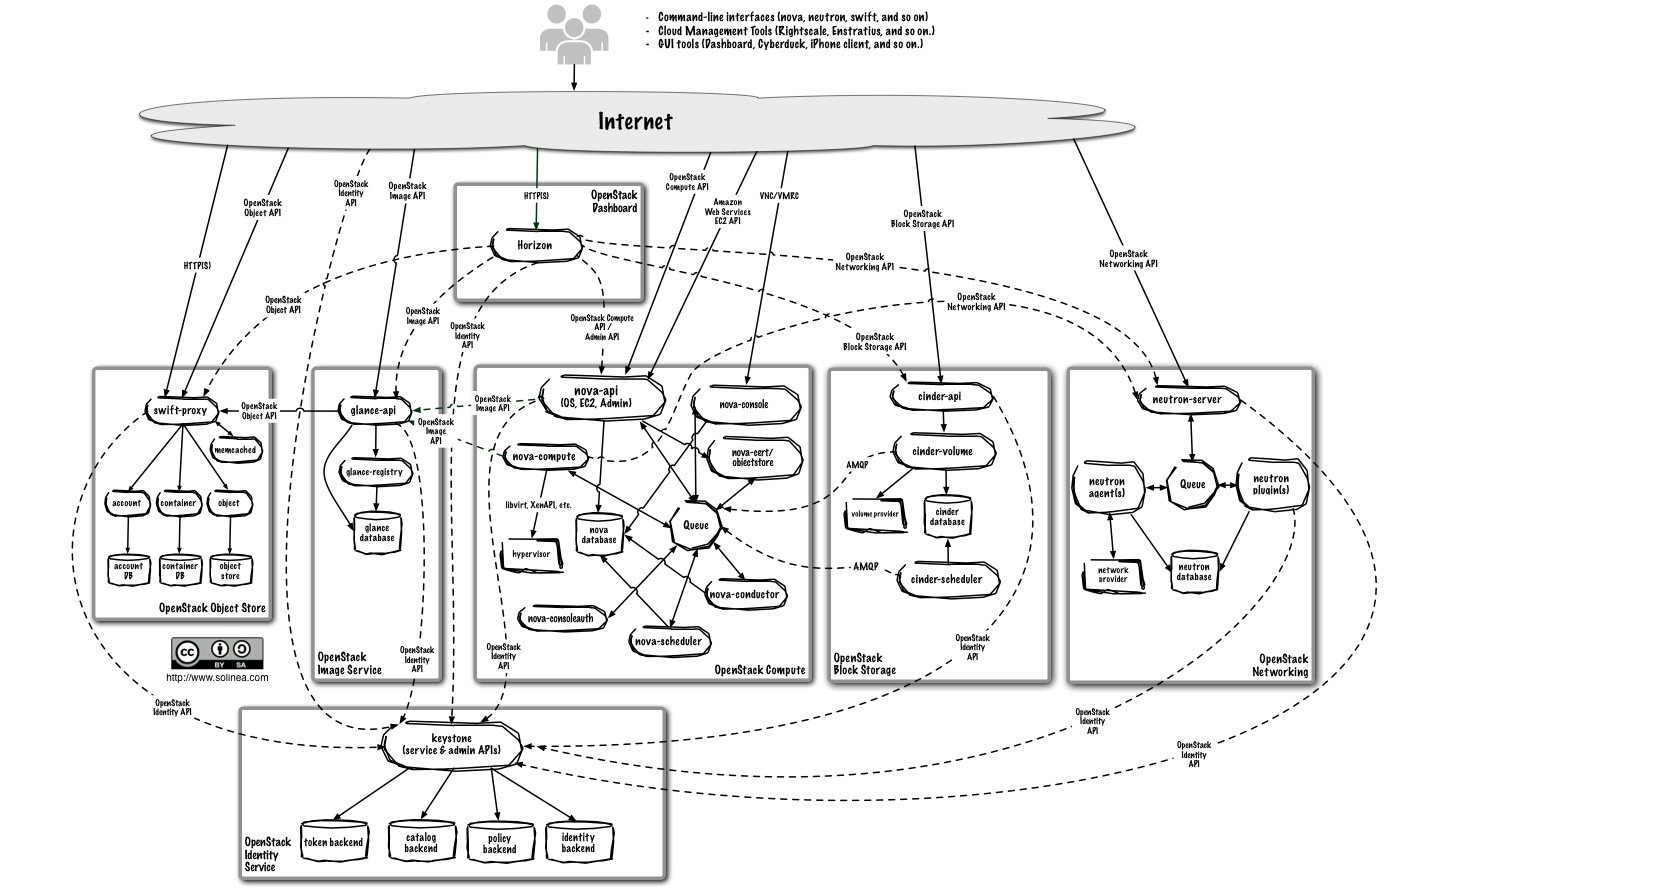
\includegraphics[width=\textwidth]{images/architecture.jpg}
    \end{center}
  \end{frame}

  \begin{frame}
    \frametitle{Quelques éléments de configuration généraux}
    \begin{itemize}
      \item Tous les composants doivent être configurés pour communiquer avec Keystone
      \item La plupart doivent être configurés pour communiquer avec MySQL et RabbitMQ
      \item Les composants découpés en plusieurs services ont souvent un fichier de configuration par service
      \item api-paste.ini contient des paramètres concernant le service API
    \end{itemize}
  \end{frame}

  \subsection[Les briques nécessaires]{Les briques nécessaires}
  \begin{frame}
    \frametitle{Système d'exploitation}
    \begin{itemize}
      \item OS Linux avec Python
      \item Historiquement : Ubuntu
      \item Red Hat s'est largement rattrapé
      \item SUSE, etc.
    \end{itemize}
  \end{frame}

  \begin{frame}
    \frametitle{Python}
    \begin{center}
      
\includegraphics{images/python-powered.png}
    \end{center}
    \begin{itemize}
      \item OpenStack est aujourd'hui compatible Python 2.7
      \item Afin de ne pas réinventer la roue, beaucoup de dépendances sont nécessaires
      \item Un travail de portage vers Python 3 est en cours
    \end{itemize}
  \end{frame}

  \begin{frame}
    \frametitle{Base de données}
    \begin{itemize}
      \item Permet de stocker la majorité des données gérées par OpenStack
      \item Chaque composant a sa propre base
      \item OpenStack utilise l'ORM Python SQLAlchemy
      \item Support théorique équivalent à celui de SQLAlchemy
      \item MySQL est l'implémentation la plus largement testée et utilisée
      \item SQLite est principalement utilisé dans le cadre de tests et démo
      \item Certains déploiements fonctionnent avec PostgreSQL
    \end{itemize}
  \end{frame}

  \begin{frame}
    \frametitle{Pourquoi l'utilisation de SQLAlchemy}
    \begin{center}
      
\includegraphics[width=10cm]{images/sqlalchemy-logo.png}
    \end{center}
    \begin{itemize}
      \item Support de multiples BDD
      \item Gestion des migrations
    \end{itemize}
    \begin{center}
      
\includegraphics{images/mysql-logo.png}
    \end{center}
  \end{frame}

  \begin{frame}
    \frametitle{Passage de messages}
    \begin{itemize}
      \item AMQP : Advanced Message Queuing Protocol
      \item Messages, file d'attente, routage
      \item Les processus OpenStack communiquent via AMQP
      \item Plusieurs implémentations possibles : Qpid, 0MQ, etc.
      \item RabbitMQ par défaut
    \end{itemize}
  \end{frame}

  \begin{frame}
  \frametitle{RabbitMQ}
    \begin{center}
      
\includegraphics{images/rabbitmq-logo.png}
    \end{center}
    \begin{itemize}
      \item RabbitMQ est implémenté en Erlang
      \item Une machine virtuelle Erlang est donc nécessaire
    \end{itemize}
  \end{frame}

  \begin{frame}
    \frametitle{"Hello world" RabbitMQ}
    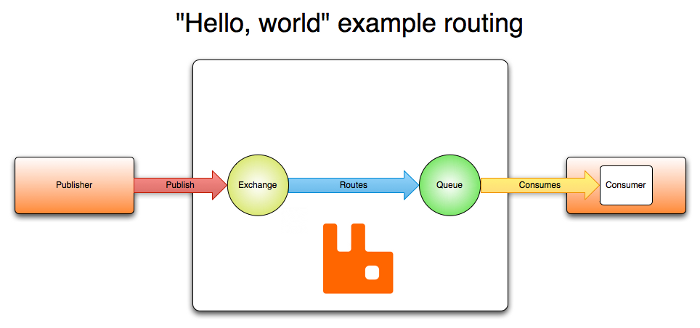
\includegraphics[width=\textwidth]{images/rabbitmq-schema.png}
  \end{frame}

  \subsection[Keystone]{Keystone : Authentification, autorisation et catalogue de services}

  \begin{frame}
    \frametitle{Principes}
    \begin{itemize}
      \item Annuaire des utilisateurs et des groupes
      \item Catalogue de services
      \item Gère l'authentification et l'autorisation
      \item Support des domaines dans l'API v3
      \item Fournit un token à l'utilisateur
    \end{itemize}
  \end{frame}

  \begin{frame}
    \frametitle{API}
    \begin{itemize}
      \item API admin : port 35357
      \item API utilisateur : port 5000
      \item Deux versions : v2 (actuelle) et v3 (future)
      \item Gère \textit{utilisateurs}, \textit{groupes}, \textit{domaines} (APIv3)
      \item Les utilisateurs ont des \textit{rôles} sur des \textit{tenants} (projets)
    \end{itemize}
  \end{frame}

  \begin{frame}
    \frametitle{Scénario d'utilisation typique}
    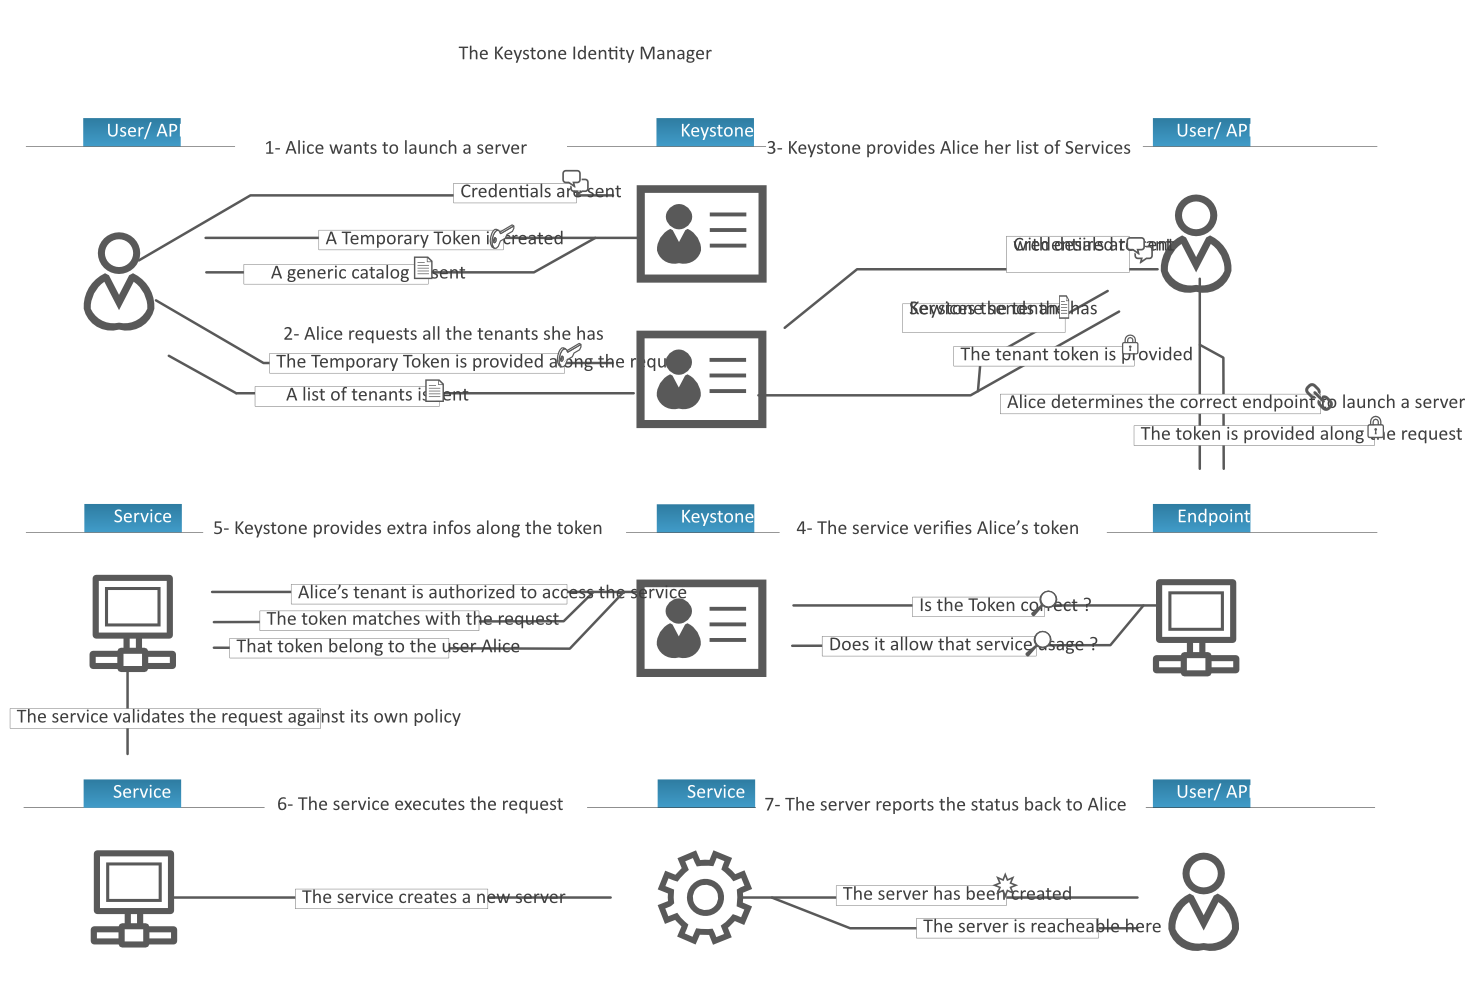
\includegraphics[width=\linewidth]{images/keystone-scenario.png}
  \end{frame}

  \begin{frame}
    \frametitle{Installation et configuration}
    \begin{itemize}
      \item Paquet : keystone
      \item Configuration d'un token ADMIN pour la configuration initiale
      \item Backends : choix de SQL ou LDAP (ou AD)
      \item Configurer les différents services
      \item Policy.json
      \item Services et endpoints
      \item Utilisateurs, groupes, domaines
    \end{itemize}
  \end{frame}

  \begin{frame}[containsverbatim]
    \frametitle{Enregistrer un service et son endpoint}
    Il faut renseigner l'existence des différents services (catalogue) dans Keystone :
    \begin{verbatim}
$ keystone service-create --name=cinderv2 --type=volumev2 \
  --description="Cinder Volume Service V2"
$ keystone endpoint-create \
  --region=myRegion
  --service-id=...
  --publicurl=http://controller:8776/v2/%\(tenant_id\)s \
  --internalurl=http://controller:8776/v2/%\(tenant_id\)s \
  --adminurl=http://controller:8776/v2/%\(tenant_id\)s
    \end{verbatim}
  \end{frame}

  \begin{frame}[containsverbatim]
    \frametitle{Tester}
\begin{verbatim}
$ keystone service-list
...
$ keystone user-list
...
$ keystone token-get
...
\end{verbatim}
  \end{frame}

  \subsection[Nova]{Nova : Compute}

  \begin{frame}
    \frametitle{Principes}
    \begin{itemize}
      \item Gère les instances
      \item IP flottantes, groupes de sécurité
      \item Les instances sont créées à partir des images fournies par Glance
      \item Les interfaces réseaux des instances sont associées à des ports Neutron
    \end{itemize}
  \end{frame}

  \begin{frame}
    \frametitle{Interactions avec les autres composants}
    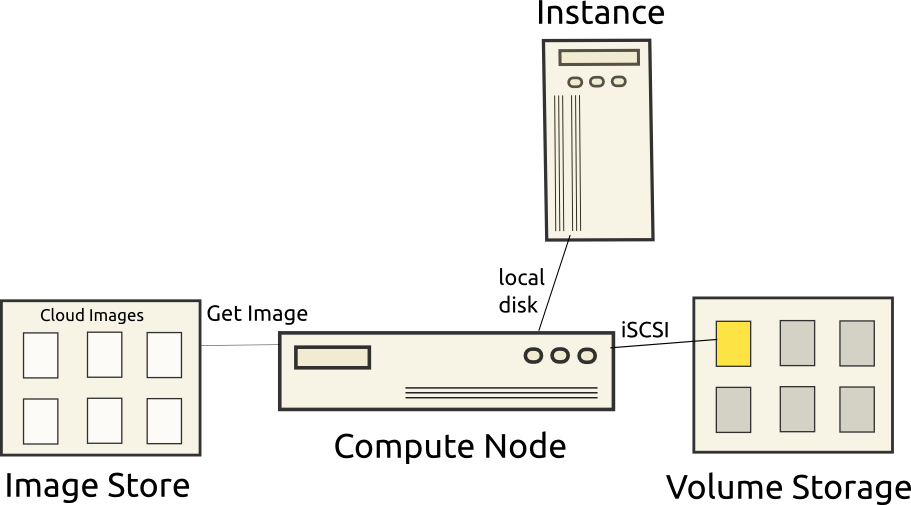
\includegraphics[width=\textwidth]{images/compute-node.png}
  \end{frame}

  \begin{frame}
    \frametitle{API}
    Gère :
    \begin{itemize}
      \item Instances
      \item Flavors (types d'instance)
      \item Security Groups (groupes de sécurité)
      \item Floating IPs (IPs flottantes)
    \end{itemize}
    Les instances sont redimensionnables et migrables d'un hôte physique à un autre.
  \end{frame}

  \begin{frame}
    \frametitle{Les groupes de sécurité}
    \begin{itemize}
      \item Équivalent à un firewall devant chaque instance
      \item Une instance peut être associée à un ou plusieurs groupes de sécurité
      \item Gestion des accès en entrée et sortie
      \item Règles par protocole (TCP/UDP/ICMP) et par port
    \end{itemize}
  \end{frame}

  \begin{frame}
    \frametitle{Rôle des flavors}
    \begin{itemize}
      \item Équivalent des "instance types" d'AWS
      \item Définit un modèle d'instance en termes de CPU, RAM, disque
    \end{itemize}
  \end{frame}

  \begin{frame}
    \frametitle{Nova api}
    \begin{itemize}
      \item Double rôle
      \item API de manipulation des instances par l'utilisateur
      \item API à destination des instances : API de metadata
      \item L'API de metadata doit être accessible à l'adresse http://169.254.169.254/
      \item L'API de metadata fournit des informations de configuration personnalisées à chacune des instances
    \end{itemize}
  \end{frame}

  \begin{frame}
    \frametitle{Nova compute}
    \begin{itemize}
      \item Exécute les machines virtuelles
      \item Tire partie de libvirt ou d'autres APIs comme XenAPI
      \item Drivers : libvirt, XenAPI, VMWare ESX, Docker
      \item Permet de récupérer les logs de la console et une console VNC
    \end{itemize}
  \end{frame}

  \begin{frame}
    \frametitle{Nova scheduler}
    \begin{itemize}
      \item Service qui distribue les demandes d'instances sur les noeuds compute
      \item Filter, Chance, Multi Scheduler
      \item Filtres, par défaut : AvailabilityZoneFilter,RamFilter,ComputeFilter
      \item Tri par poids, par défaut : RawWeigher
    \end{itemize}
  \end{frame}

  \begin{frame}
    \frametitle{Le scheduler Nova en action}
    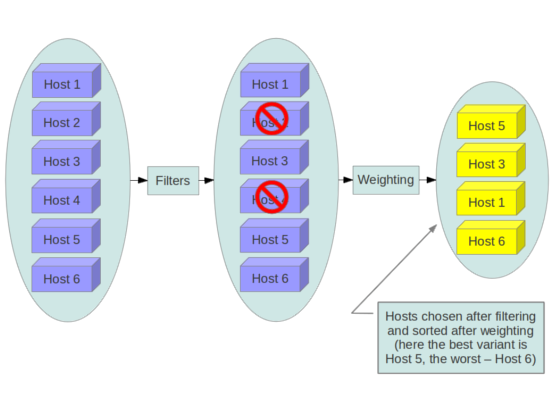
\includegraphics[width=\textwidth]{images/scheduling-schema.png}
  \end{frame}

  \begin{frame}
    \frametitle{Nova conductor}
    \begin{itemize}
      \item Service facultatif qui améliore la sécurité
      \item Fait office de proxy entre les noeuds compute et la BDD
      \item Les noeuds compute, vulnérables, n'ont donc plus d'accès à la BDD
    \end{itemize}
  \end{frame}

  \begin{frame}[containsverbatim]
    \frametitle{Tester}
\begin{verbatim}
$ nova list
...
$ nova create
...
\end{verbatim}
  \end{frame}

  \subsection[Glance]{Glance : Registre d'images}

  \begin{frame}
    \frametitle{Principes}
    \begin{itemize}
      \item Registre d'images (et des snapshots)
      \item Propriétés sur les images
      \item Est utilisé par Nova pour démarrer des instances
      \item Peut utiliser Swift comme back-end de stockage
    \end{itemize}
  \end{frame}

  \begin{frame}
    \frametitle{Propriétés des images dans Glance}
    L'utilisateur peut définir un certain nombre de propriétés dont certaines seront utilisées lors de l'instanciation
    \begin{itemize}
      \item Type d'image
      \item Architecture
      \item Distribution
      \item Version de la distribution
      \item Espace disque minimum
      \item RAM minimum
      \item Publique ou non
    \end{itemize}
  \end{frame}

  \begin{frame}
    \frametitle{Types d'images}
    Glance supporte un large éventail de types d'images, limité par le support de l'hyperviseur sous-jacent à Nova
    \begin{itemize}
      \item raw
      \item qcow2
      \item ami
      \item vmdk
      \item iso
    \end{itemize}
  \end{frame}

  \begin{frame}
    \frametitle{Backends}
    \begin{itemize}
      \item Swift ou S3
      \item Ceph
      \item HTTP
      \item Répertoire local
    \end{itemize}
  \end{frame}

  \begin{frame}
    \frametitle{Installation}
    \begin{itemize}
      \item Paquet glance-api : fournit l'API
      \item Paquet glance-registry : démon du registre d'images en tant que tel
    \end{itemize}
  \end{frame}

  \begin{frame}[containsverbatim]
    \frametitle{Tester}
\begin{verbatim}
$ glance image-list
...
$ glance image-create
...
\end{verbatim}
  \end{frame}

  \subsection[Neutron]{Neutron : Réseau en tant que service}

  \begin{frame}
    \frametitle{Principes}
    \begin{itemize}
      \item SDN
      \item Auparavant Quantum et nova-network
      \item neutron-server : fournit l'API
      \item Agent DHCP : fournit le service de DHCP pour les instances
      \item Agent L3 : gère la couche 3 du réseau, le routage
      \item Plugin : OpenVSwitch par défaut, d'autres implémentations libres/propriétaires, logicielles/matérielles existent
    \end{itemize}
  \end{frame}

  \begin{frame}
    \frametitle{Fonctionnalités supplémentaires}
    Outre les fonctions réseau de base niveaux 2 et 3, Neutron peut fournir d'autres services :
    \begin{itemize}
      \item Load Balancing (HAProxy, ...)
      \item Firewall (vArmour, ...) : différe des groupes de sécurité
      \item VPN (Openswan, ...) : permet d'accéder à un réseau privé sans IP flottantes
    \end{itemize}
    Ces fonctionnalités se basent également sur des plugins
  \end{frame}

  \begin{frame}
    \frametitle{API}
    L'API permet notamment de manipuler ces ressources
    \begin{itemize}
      \item Réseau : niveau 2
      \item Subnet : niveau 3
      \item Port
    \end{itemize}
    Les ports peuvent correspondre à des interfaces d'instance
  \end{frame}

  \begin{frame}
    \frametitle{Plugins ML2}
    \begin{itemize}
      \item Modular Layer 2
      \item OpenVSwitch
      \item OpenDaylight
      \item Contrail, OpenContrail
      \item Nuage Networks
      \item cf. OpenFlow
    \end{itemize}
  \end{frame}

  \begin{frame}
    \frametitle{Implémentation}
    \begin{itemize}
      \item Neutron tire partie des namespaces réseaux du noyau Linux pour permettre l'IP overlapping
      \item Le proxy de metadata est un composant qui permet aux instances isolées dans leur réseau de joindre l'API de metadata fournie par Nova
    \end{itemize}
  \end{frame}

  \begin{frame}
    \frametitle{Schéma}
    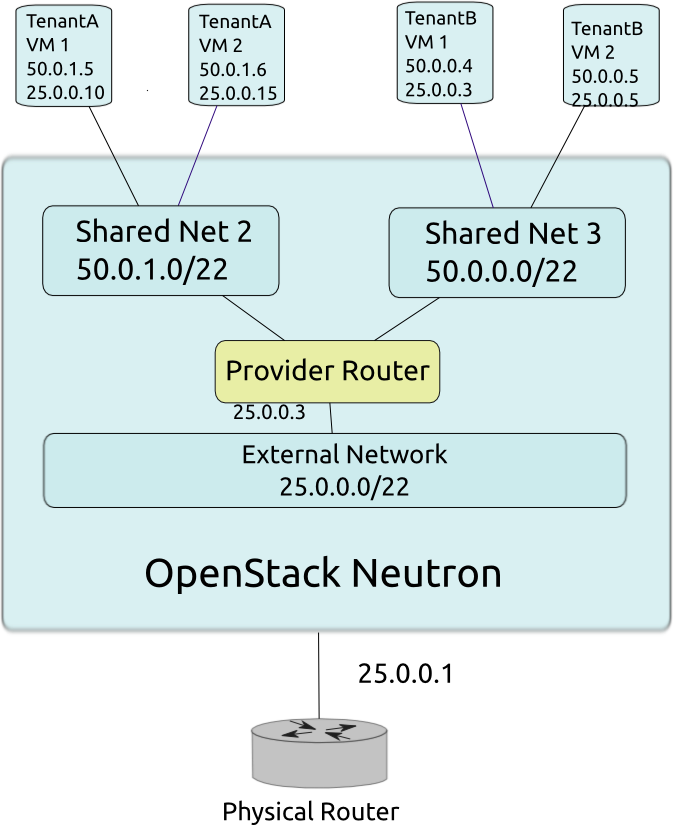
\includegraphics[width=\textwidth,height=\textheight]{images/neutron-schema.png}
  \end{frame}

  \subsection[Cinder]{Cinder : Stockage block}

  \begin{frame}
    \frametitle{Principes}
    \begin{itemize}
      \item Auparavant nova-volume
      \item Fournit des volumes (stockage block) attachables aux instances
      \item Gère différents types de volume
      \item Gère snapshots et backups de volumes
      \item Attachement via iSCSI par défaut
    \end{itemize}
  \end{frame}

  \begin{frame}
    \frametitle{Du stockage partagé ?}
    \begin{itemize}
      \item Cinder n'est \textbf{pas} une solution de stockage partagé comme NFS
      \item OpenStack (tout comme AWS) ne fournit pas de solution \textit{NFS as a Service}
      \item Cf. le projet Manila
    \end{itemize}
  \end{frame}

  \begin{frame}
    \frametitle{Utilisation}
    \begin{itemize}
      \item Volume supplémentaire (et stockage persistant) sur une instance
      \item Boot from volume : l'OS est sur le volume
      \item Fonctionnalité de backup vers un object store (Swift ou Ceph)
    \end{itemize}
  \end{frame}

  \begin{frame}
    \frametitle{Installation}
    \begin{itemize}
      \item Paquet cinder-api : fournit l'API
      \item Paquet cinder-volume : création et gestion des volumes
      \item Paquet cinder-scheduler : distribue les demandes de création de volume
      \item Paquet cinder-backup : backup vers un object store
    \end{itemize}
  \end{frame}

  \begin{frame}
    \frametitle{Backends}
    \begin{itemize}
      \item Utilisation de plusieurs backends en parallèle possible
      \item LVM (par défaut)
      \item GlusterFS
      \item Ceph
      \item Systèmes de stockage propriétaires type NetApp
    \end{itemize}
  \end{frame}

  \subsection[Horizon]{Horizon : Dashboard web}

  \begin{frame}
    \frametitle{Principes}
    \begin{itemize}
      \item Utilise les APIs existantes pour fournir une interface
      \item Horizon est un module Django
      \item OpenStack Dashboard est l'implémentation officielle de ce module
    \end{itemize}
    \begin{center}
      
\includegraphics[width=8cm]{images/django-logo.png}
    \end{center}
  \end{frame}

  \begin{frame}
    \frametitle{Configuration}
    \begin{itemize}
      \item local\_settings.py
      \item Les services apparaissent dans Horizon s'ils sont répertoriés dans le catalogue de services de Keystone
    \end{itemize}
  \end{frame}

  \begin{frame}
    \frametitle{Utilisation}
    \begin{itemize}
      \item Une zone "admin" restreinte
      \item Une interface par tenant
    \end{itemize}
  \end{frame}

  \subsection[Swift]{Swift : Stockage objet}

  \begin{frame}
    \frametitle{Principes}
    \begin{itemize}
      \item SDS : Software Defined Storage
      \item Utilisation de commodity hardware
      \item Théorème CAP : on en choisit deux
      \item Accès par les APIs
      \item Architecture totalement acentrée
      \item Pas de base de données centrale
    \end{itemize}
  \end{frame}

  \begin{frame}
    \frametitle{Implémentation}
    \begin{itemize}
      \item Proxy : serveur API par lequel passent toutes les requêtes
      \item Object server : serveur de stockage
      \item Container server : maintient des listes d'objects dans des containers
      \item Account server : maintient des listes de containers dans des accounts
      \item Chaque objet est répliqué n fois (3 par défaut)
    \end{itemize}
  \end{frame}

  \begin{frame}
    \frametitle{Le ring}
    \begin{itemize}
      \item Problème : comment décider quelle donnée va sur quel object server
      \item Le ring est découpé en partitions
      \item On situe chaque donnée dans le ring afin de déterminer sa partition
      \item Une partition est associée à plusieurs serveurs
    \end{itemize}
  \end{frame}

  \begin{frame}
    \frametitle{Schéma}
    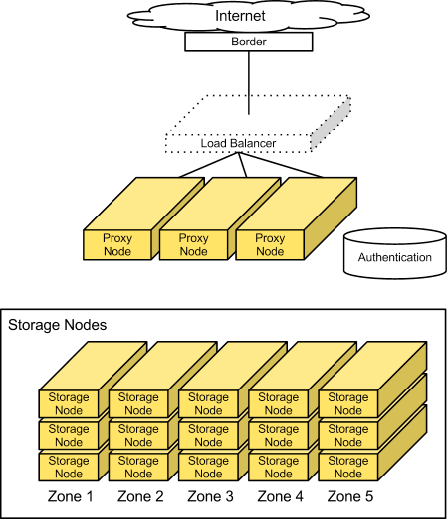
\includegraphics[width=\textwidth,height=\textheight]{images/swift-schema.png}
  \end{frame}

  \subsection[Ceilometer]{Ceilometer : Collecte de métriques}

  \begin{frame}
    \frametitle{Surveiller l'utilisation de son infrastructure avec Ceilometer}
    \begin{itemize}
      \item Indexe différentes métriques concernant l'utilisation des différents services du cloud
      \item Fournit des APIs permettant de récupérer ces données
      \item Base pour construire des outils de facturation
      \item Utilise MongoDB (par défaut) pour le stockage
    \end{itemize}
  \end{frame}

  \subsection[Heat]{Heat : Orchestration des ressources}

  \begin{frame}
    \frametitle{Orchestrer son infrastructure avec Heat}
    \begin{itemize}
      \item Équivalent d'Amazon Cloud Formation
      \item Orchestrer les ressources compute, storage, network, etc.
      \item Doit se coupler avec cloud-init\pause
      \item Description de son infrastructure dans un fichier template, format JSON (CFN) ou YAML (HOT)
    \end{itemize}
  \end{frame}

  \begin{frame}
    \frametitle{Autoscaling avec Heat}
    Heat implémente la fonctionnalité d'autoscaling
    \begin{itemize}
      \item Se déclenche en fonction des alarmes produites par Ceilometer
      \item Entraine la création de nouvelles instances
    \end{itemize}
  \end{frame}

  \begin{frame}[containsverbatim]
    \frametitle{Un template HOT}
\begin{verbatim}
heat_template_version: 2013-05-23

description: Simple template to deploy a single compute instance

resources:
  my_instance:
    type: OS::Nova::Server
    properties:
      key_name: my_key
      image: F18-x86_64-cfntools
      flavor: m1.small
\end{verbatim}
  \end{frame}

  \begin{frame}
    \frametitle{Fonctionnalités avancées de Heat}
    \begin{itemize}
      \item Nested stacks
      \item Environments
      \item Providers
    \end{itemize}
  \end{frame}

  \subsection[Trove]{Trove : Database as a Service}

  \begin{frame}
    \frametitle{Principe}
    \begin{itemize}
      \item Fournit des bases de données relationnelles, à la AWS RDS
      \item A vocation à supporter des bases NoSQL aussi
      \item Gère notamment MySQL comme back-end
      \item Se repose sur Nova pour les instances dans lesquelles se fait l'installation d'une BDD
    \end{itemize}
  \end{frame}

  \begin{frame}
    \frametitle{Services}
    \begin{itemize}
      \item trove-api : API
      \item trove-taskmanager : gère les instances BDD
      \item trove-guestagent : agent interne à l'instance
    \end{itemize}
  \end{frame}

  \subsection[Designate]{Designate : DNS as a Service}

  \begin{frame}
    \frametitle{Principe}
    \begin{itemize}
      \item Équivalent d'AWS Route 53
      \item Gère différents backends : BIND, etc.
    \end{itemize}
  \end{frame}

  \subsection[Les autres]{Quelques autres composants intéressants}

  \begin{frame}
    \frametitle{Ironic}
    \begin{itemize}
      \item Anciennement Nova bare-metal
      \item Permet le déploiement d'instance sur des machines physiques (plutôt que VMs)
      \item Repose sur des technologies telles que PXE, TFTP
    \end{itemize}
  \end{frame}

  \begin{frame}
    \frametitle{Oslo, ou OpenStack common}
    \begin{itemize}
      \item Oslo contient le code commun à plusieurs composants d'OpenStack
      \item Son utilisation est transparente pour le déployeur
    \end{itemize}
  \end{frame}

  \begin{frame}
    \frametitle{rootwrap}
    \begin{itemize}
      \item Wrapper pour l'utilisation de commandes en root
      \item Configuration au niveau de chaque composant qui l'utilise
      \item Permet d'écrire des filtres sur les commandes
    \end{itemize}
  \end{frame}

  \begin{frame}
    \frametitle{TripleO}
    \begin{itemize}
      \item OpenStack On OpenStack
      \item Objectif : pouvoir déployer un cloud OpenStack (overcloud) à partir d'un cloud OpenStack (undercloud)
      \item Autoscaling du cloud lui-même : déploiement de nouveaux noeuds compute lorsque cela est nécessaire
      \item Fonctionne conjointement avec Ironic pour le déploiement bare-metal
    \end{itemize}
  \end{frame}

  \begin{frame}
    \frametitle{Tempest}
    \begin{itemize}
      \item Suite de tests d'un cloud OpenStack
      \item Effectue des appels à l'API et vérifie le résultat
      \item Est très utilisé par les développeurs via l'intégration continue
      \item Le déployeur peut utiliser Tempest pour vérifier la bonne conformité de son cloud
    \end{itemize}
  \end{frame}

  \subsection[Déployer en production]{Bonnes pratiques pour un déploiement en production}

  \begin{frame}
    \frametitle{Quels composants dois-je installer ?}
      \begin{itemize}
        \item Keystone est indispensable
        \item L'utilisation de Nova va de paire avec Glance et Neutron
        \item Cinder s'avérera souvent utile
        \item Ceilometer et Heat vont souvent ensemble
        \item Swift est indépendant des autres composants
      \end{itemize}
  \end{frame}

  \begin{frame}
    \frametitle{Penser dès le début aux choix structurants}
    \begin{itemize}
      \item Distribution et méthode de déploiement
      \item Hyperviseur
      \item Réseau : quelle architecture et quels drivers
      \item Politique de mise à jour
    \end{itemize}
  \end{frame}

  \begin{frame}
    \frametitle{Les différentes méthodes d'installation}
    \begin{itemize}
      \item DevStack est à oublier pour la production
      \item TripleO est encore trop jeune
      \item Le déploiement à la main comme vu précédemment n'est pas recommandé car peu maintenable
      \item Distributions OpenStack packagées et prêtes à l'emploi
      \item Distributions classiques et gestion de configuration
    \end{itemize}
  \end{frame}

  \begin{frame}
    \frametitle{Assigner des rôles aux machines}
    Beaucoup de documentations font référence à ces rôles :
    \begin{itemize}
      \item Controller node : APIs, BDD, AMQP
      \item Network node : Routeur
      \item Compute node : Hyperviseur
    \end{itemize}
    Ce modèle simplifié n'est pas HA.
  \end{frame}

  \begin{frame}
    \frametitle{Haute disponbilité}
    Haut disponibilité de l'IaaS
    \begin{itemize}
      \item MySQL, RabbitMQ : HA classique (Galera, Clustering)
      \item Les services APIs sont stateless et HTTP : scale out et load balancers
      \item La plupart des autres services OpenStack sont capables de scale out également
    \end{itemize}
    Guide HA : \url{http://docs.openstack.org/high-availability-guide/content/}
  \end{frame}

  \begin{frame}
    \frametitle{Haute disponibilité de l'agent L3 de Neutron}
    \begin{itemize}
      \item Plusieurs solutions possibles
    \end{itemize}
  \end{frame}

  \begin{frame}
    \frametitle{Considérations pour une environnement de production}
    \begin{itemize}
      \item Des URLs uniformes pour toutes les APIs : utiliser un reverse proxy
      \item Utilisation des quotas
      \item Prévoir les bonnes volumétries, notamment pour les données Ceilometer
      \item Monitoring
      \item Backup
    \end{itemize}
    Guide Operations : \url{http://docs.openstack.org/trunk/openstack-ops/content/}
  \end{frame}

  \begin{frame}
  \frametitle{Découpage réseau}
    \begin{itemize}
      \item Management network : réseau d'administration
      \item Data network : réseau pour la communication inter instances
      \item External network : réseau externe, dans l'infrastructure réseau existante
      \item API network : réseau contenant les endpoints API
    \end{itemize}
  \end{frame}

  \begin{frame}
    \frametitle{Considérations liées à la sécurité}
    \begin{itemize}
      \item Indispensable : HTTPS sur l'accès des APIs à l'extérieur
      \item Sécurisation des communications MySQL et RabbitMQ
      \item Un accès MySQL par base et par service
      \item Un utilisateur Keystone par service
      \item Limiter l'accès en lecture des fichiers de configuration (mots de passe, token)
      \item Veille sur les failles de sécurité : OSSA
      Guide sécurité : \url{http://docs.openstack.org/security-guide/content/}
    \end{itemize}
  \end{frame}

  \begin{frame}
    \frametitle{Segmenter son cloud}
    \begin{itemize}
      \item Host aggregates : machines physiques avec des caractéristiques similaires
      \item Availability zones : machines dépendantes d'une même source électrique, d'un même switch, d'un même DC, etc.
      \item Regions : chaque région a son API
      \item Cells : permet de regrouper plusieurs cloud différents sous une même API
    \end{itemize}
  \end{frame}

  \begin{frame}
    \frametitle{Host aggregates / agrégats d'hôtes}
    \begin{itemize}
      \item L'administrateur définit des agrégats via l'API
      \item 1 agrégat $\equiv$ 1 point commun, ex : GPU
      \item L'utilisateur peut choisir un agrégat à la création d'instance
    \end{itemize}
  \end{frame}

  \begin{frame}
    \frametitle{Availability zones / zones de disponibilité}
    \begin{itemize}
      \item Groupe d'hôtes
      \item Découpage en termes de disponibilité : Rack, Datacenter, etc.
      \item L'utiliser peut choisir une zone de disponibilité
      \item L'utilisateur peut demander à ce que des instances soient démarrées dans une même zone, ou au contraire dans des zones différentes
    \end{itemize}
  \end{frame}

  \begin{frame}
    \frametitle{Régions}
    \begin{itemize}
      \item Équivalent des régions d'AWS
      \item Un service peut avoir différents endpoints dans différentes régions
      \item Chaque région est autonome
      \item Cas d'usage : cloud de grande ampleur (comme certains clouds publics)
    \end{itemize}
  \end{frame}

  \begin{frame}
    \frametitle{Cellules / Cells}
    \begin{itemize}
      \item Fonctionnalité de Nova uniquement
      \item Un seul nova-api devant plusieurs cellules
      \item Chaque cellule a sa propre BDD et file de messages
      \item Ajoute un niveau de scheduling (choix de la cellule)
    \end{itemize}
  \end{frame}

  \begin{frame}
    \frametitle{Packaging d'OpenStack - Ubuntu}
    \begin{itemize}
      \item Le packaging est fait dans de multiples distributions, RPM, DEB et autres\pause
      \item Ubuntu est historiquement la plateforme de référence pour le développement d'OpenStack
      \item Le packaging dans Ubuntu suit de près le développement d'OpenStack, et des tests automatisés sont réalisés
      \item Canonical fournit la Ubuntu Cloud Archive, qui met à disposition la dernière version d'OpenStack pour la dernière Ubuntu LTS
    \end{itemize}
  \end{frame}

  \begin{frame}
    \frametitle{Ubuntu Cloud Archive}
    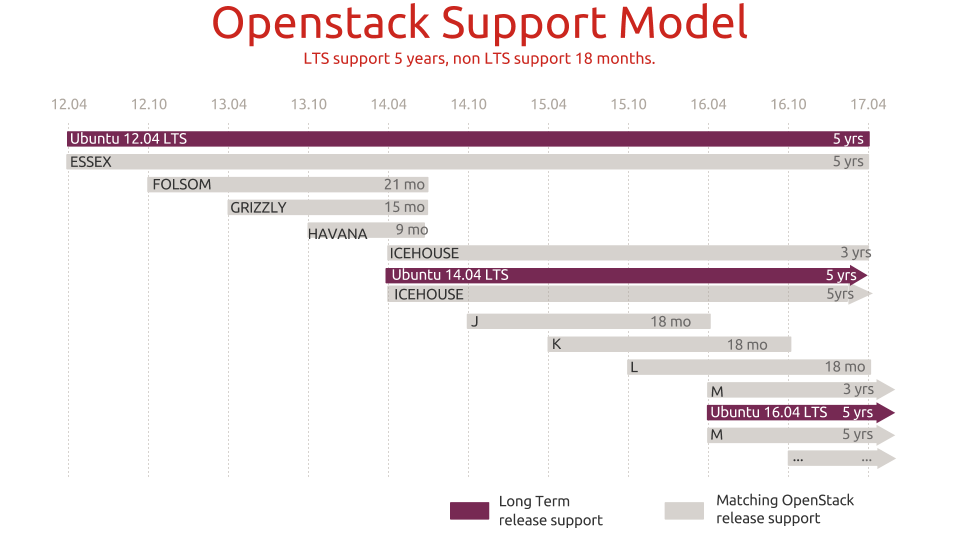
\includegraphics[width=\textwidth]{images/ubuntu-cloud-archive.png}
  \end{frame}

  \begin{frame}
    \frametitle{Packaging d'OpenStack dans les autres distributions}
    \begin{itemize}
      \item OpenStack est intégré dans les dépôts officiels de Debian
      \item Red Hat propose RHOS/RDO
      \item Comme Ubuntu, le cycle de release de Fedora est synchronisé avec celui d'OpenStack
    \end{itemize}
  \end{frame}

  \begin{frame}
    \frametitle{Les distributions OpenStack}
    \begin{itemize}
      \item StackOps
      \item Mirantis
      \item HP
      \item etc.
    \end{itemize}
  \end{frame}

  \begin{frame}
    \frametitle{Déploiement bare metal}
    \begin{itemize}
      \item Le déploiement des hôtes physiques OpenStack peut se faire à l'aide d'outils dédiés\pause
      \item Canonical/Ubuntu propose MaaS : Metal as a Service
      \item Dell propose Crowbar
      \item eDeploy (eNovance)
    \end{itemize}
  \end{frame}

  \begin{frame}
    \frametitle{Gestion de configuration}
    \begin{itemize}
      \item Puppet, Chef, CFEngine, Saltstack, Ansible, etc.\pause
      \item Ces outils peuvent aider à déployer le cloud OpenStack
      \item ... mais aussi à gérer les instances (section suivante)
    \end{itemize}
  \end{frame}

  \begin{frame}
    \frametitle{Modules Puppet}
    \begin{itemize}
      \item Puppet Labs maintient (avec d'autres) des modules pour déployer OpenStack
      \item \url{https://forge.puppetlabs.com/puppetlabs/openstack}
    \end{itemize}
  \end{frame}

  \begin{frame}
    \frametitle{Déploiement continu}
    \begin{itemize}
      \item OpenStack maintient un master (trunk) toujours stable
      \item Possibilité de déployer au jour le jour le master (CD: \textit{Continous Delivery})
      \item Nécessite la mise en place d'une infrastructure importante
      \item Facilite les mises à jour entre versions majeures
    \end{itemize}
  \end{frame}

  \subsection[Problèmes]{Faire face aux problèmes}

  \begin{frame}
    \frametitle{Les réflexes en cas d'erreur ou de comportement erroné}
    \begin{itemize}
      \item Travaille-t-on sur le bon tenant ?
      \item Est-ce que l'API renvoie une erreur ? (le dashboard peut cacher certaines informations)
      \item Si nécessaire d'aller plus loin :
        \begin{itemize}
          \item Regarder les logs sur le cloud controller (/var/log/\textless composant\textgreater/*.log)
          \item Regarder les logs sur le compute node et le network node si le problème est spécifique réseau/instance
          \item Éventuellement modifier la verbosité des logs dans la configuration
        \end{itemize}
    \end{itemize}
  \end{frame}

  \begin{frame}
    \frametitle{Est-ce un bug ?}
    \begin{itemize}
      \item Si le client CLI crash, c'est un bug\pause
      \item Si le dashboard web affiche une erreur 500, c'est peut-être un bug\pause
      \item Si les logs montrent une stacktrace Python, c'est un bug\pause
      \item Sinon, à vous d'en juger
    \end{itemize}
  \end{frame}
